\documentclass[
fontsize=12pt,					% Schriftgröße
paper=a4,						% Papierformat
twoside=true, 					% einseitiges (false) oder zweiseitiges (true) Dokument
listof=totoc, 					% Tabellen- und Abbildungsverzeichnis ins Inhaltsverzeichnis
bibliography=totoc,				% Literaturverzeichnis ins Inhaltsverzeichnis aufnehmen
titlepage, 						% Titlepage-Umgebung statt \maketitle
headsepline, 					% horizontale Linie unter Kolumnentitel
%abstracton,					% Überschrift beim Abstract einschalten, Abstract muss dazu in {abstract}-Umgebung stehen
DIV=12,							% Satzspiegeleinstellung, 12 ist Standar bei KOMA
BCOR=6mm,						% Bindekorrektur, die den Seitenspiegel um 3mm nach rechts verschiebt,
cleardoublepage=empty,			% Stil einer leeren eingefügten Seite bei Kapitelwechsel
parskip,							% Absatzabstand bei Absatzwechsel einfügen
ngerman
]{scrartcl}

\usepackage[setspace=false]{scrhack}
\usepackage[utf8]{inputenc} 	% ermöglicht die direkte Eingabe von Umlauten
\usepackage[T1]{fontenc} 		% Ausgabe aller zeichen in einer T1-Codierung (wichtig für die Ausgabe von Umlauten!)
\usepackage{babel} 	% deutsche Trennungsregeln und Übersetzung der festcodierten Überschriften
\renewcaptionname{ngerman}{\contentsname}{Inhaltsverzeichnis}
\renewcaptionname{ngerman}{\bibname}{Literaturverzeichnis}
\setlength{\parindent}{0ex} 	% bei neuem Abschnitt nicht einrücken

\newcommand{\lowrule}{%
	\leavevmode \kern.06em\vbox{\hrule width.5em}}

\usepackage{siunitx}			% Vereinfachte Eingabe von Einheiten in Formeln
\sisetup{
	number-unit-product = \;,
	inter-unit-product = \:,
	exponent-product = \cdot,
	output-decimal-marker = {,}
}

\usepackage{graphicx}  			% Einbinden von Grafiken erlauben
\usepackage[format=hang,		% Formatierungen von Unter- / Überschriften
font=normal,
labelfont=bf,
justification=RaggedRight,
singlelinecheck=true,
aboveskip=1mm
]{caption}

\usepackage[backend=biber, %% Hilfsprogramm "biber" beim Compilieren nutzen (statt "biblatex" oder "bibtex")
style=numeric, %% Zitierstil (siehe Dokumentation)
natbib=true, %% Bereitstellen von natbib-kompatiblen Zitierkommandos
hyperref=true, %% hyperref-Paket verwenden, um Links zu erstellen
]{biblatex}

\usepackage{pdfpages}

\usepackage{enumitem}			% Erlaubt Änderung der Nummerierung in der Umgebung enumerate

\usepackage{amsmath}			% Ergänzungen für Formeln
\usepackage{textcomp} 			% zum Einsatz von Eurozeichen u. a. Symbolen
\usepackage{eurosym}			% bessere Darstellung Euro-Symbol mit \euro

\usepackage[					% Einstellunge Paket hyperref
hyperfootnotes=false,			% im pfd-Output Fußnoten nicht verlinken
hidelinks						% Entfernen von farbigen Umrandungen der Links
]{hyperref}

\usepackage[					% Einstellungen für Fußnoten
bottom,							% Ausrichtung unten
multiple,						% Trennung durch Seperator bei mehreren Fußnoten
hang,
marginal
]{footmisc}

\usepackage{calc}				% Paket zum Berechnen von Längen z.B. 0.8\linewidth

\usepackage{xcolor} 			% einfache Verwendung von Farben in nahezu allen Farbmodellen

\usepackage{listings}			% Darstellung von Quellcode mit den Umgebungen {lstlisting}, \lstinline und \lstinputlisting
\lstset{literate=				% Damit können Umlaute innerhalb Listings geschrieben werden
	{Ö}{{\"O}}1
	{Ä}{{\"A}}1
	{Ü}{{\"U}}1
	{ß}{{\ss}}1
	{ü}{{\"u}}1
	{ä}{{\"a}}1
	{ö}{{\"o}}1
}
\definecolor{mygreen}{rgb}{0,0.6,0}
\definecolor{mygray}{rgb}{0.5,0.5,0.5}
\definecolor{mymauve}{rgb}{0.58,0,0.82}
\lstset{ %
	backgroundcolor=\color{white},   % choose the background color; you must add \usepackage{color} or \usepackage{xcolor}; should come as last argument
	basicstyle=\footnotesize,        % the size of the fonts that are used for the code
	breakatwhitespace=false,         % sets if automatic breaks should only happen at whitespace
	breaklines=true,                 % sets automatic line breaking
	captionpos=t,                    % sets the caption-position to (b) bottom or (t) top
	commentstyle=\color{mygreen},    % comment style
	deletekeywords={...},            % if you want to delete keywords from the given language
	escapeinside={\%*}{*)},          % if you want to add LaTeX within your code
	escapeinside={(*@}{@*)},
	extendedchars=true,              % lets you use non-ASCII characters; for 8-bits encodings only, does not work with UTF-8
	frame=none,	                   	% "single" adds a frame around the code; "none"
	keepspaces=true,                 % keeps spaces in text, useful for keeping indentation of code (possibly needs columns=flexible)
	keywordstyle=\color{blue},       % keyword style
	language=[LaTeX]TeX,             % the language of the code
	morekeywords={*,nomenclature},   % if you want to add more keywords to the set
	numbers=left,                    % where to put the line-numbers; possible values are (none, left, right)
	numbersep=5pt,                   % how far the line-numbers are from the code
	numberstyle=\tiny\color{mygray}, % the style that is used for the line-numbers
	rulecolor=\color{black},         % if not set, the frame-color may be changed on line-breaks within not-black text (e.g. comments (green here))
	showspaces=false,                % show spaces everywhere adding particular underscores; it overrides 'showstringspaces'
	showstringspaces=false,          % underline spaces within strings only
	showtabs=false,                  % show tabs within strings adding particular underscores
	stepnumber=1,                    % the step between two line-numbers. If it's 1, each line will be numbered
	stringstyle=\color{mymauve},     % string literal style
	tabsize=2,	                   % sets default tabsize to 2 spaces
	title=\lstname                   % show the filename of files included with \lstinputlisting; also try caption instead of title
}

% Folgende Zeilen definieren Abkürzungen, um Befehle schneller eingeben zu können
\newcommand{\ua}{\mbox{u.\,a.\ }}
\newcommand{\zB}{\mbox{z.\,B.\ }}
\newcommand{\bs}{$\backslash$}
\newcommand*\diff{\mathop{}\!\mathrm{d}}	% Differentialzeichen
\newcommand*\Diff[1]{\mathop{}\!\mathrm{d^#1}} % Differentialzeichen höherer Ableitung
\newcommand*\jj{\mathop{}\!\mathrm{j}}	% Komplexe Zahl j

% Folgende Zeilen weden benötigt, um Tikz und PGF-Plot-Grafiken einzubinden
\usepackage{pgfplots}
\usepackage{pgfplotstable}
\pgfplotsset{compat=newest,width=0.6\linewidth}
\usepgfplotslibrary{smithchart}
\usepackage{tikz}						% Tikz sollte nach Listings Pakete geladen werden.
\usetikzlibrary{arrows}

\hyphenation{Schrift-ar-ten}

\BeforeClosingMainAux{% siehe KOMA-Script-Anleitung
	\addcontentsline{toc}{chapter}{\indexname}\stepcounter{page}
}

%opening
\title{DeepLearning}
\author{Tim Lucas Halt}

\begin{document}

\maketitle

\begin{abstract}

Sehr kurz

\end{abstract}

\section{Methodik}

Mein Ziel war in einen der drei vorlesungsbegleitende Benchmarks zu führen und die Anstrengungen vorerst auf dieses Ziel zu legen.

Dafür habe ich mich in der ersten Woche in alle drei Richtungen, maximale Genauigkeit, minimale Labels und minimale Parameter probiert.

Zielerreicht wurde mit dem Netzt welches in \autoref{sec:basis} vorgestellt wurde. Eine kombination von verschiedensten quellen zusammengedrafen und mit etwas glück auf 99,47 \% gebracht

Die weitere Verbesserung wollte ich vor allem automatisieren.

Dafür habe ich Kostenlose Grafikkarten von Kaggle (30 Stunden die Woche) und Colab (12 Stunden am Tag) genutzt. 

Im ersten Schritt wollte ich die Wahl der Hyperparemter meines optimieren. dafür habe ich verschiedene Kombinationen mit weights \& biases sweepen und tracken lassen


\section{Basis -  }
\label{sec:basis}

Das Ausgangsnetz von dem die Untersuchungen ausgehen ist in \autoref{basis} dargestellt. Es hat etwa 62-tausend Parameter und wurde mit dem vollständigen Trainingsdatensatz (60000 Label) trainiert.

Kompeliert mit dem Adam Optimizer mit einer Learining rate von 0.003 Mit einer Batch-Size von 512 ereichte das Modell nach 100 Epochen 99,47  \% val\_accuracy

\begin{lstlisting}[language=Python, caption=Python-Code, label=basis]
	InputLayer(input_shape=(28,28,1)),
	Conv2D(filter=28, kernel_size=5, padding='same', activation='relu'),
	MaxPooling2D(2,2),
	Conv2D(filter=16, kernel_size=5, padding='same', activation='relu'),
	MaxPooling2D(2,2),
	layers.Dropout(0.2),
	layers.Flatten(),
	layers.Dropout(0.2),
	layers.Dense(64, kernel_regularizer = tf.keras.regularizers.l2(0.07), activation = 'relu'),
	GaussianNoise(0.1),
	Dense(10, activation='softmax')
\end{lstlisting}

Erkenntnis learning rate und batchsize haben einfluss, aber wie?

Sweep, um filteranzah in conv2d layer zu testen, sowie die des zweitletzten dense layers zu verbessern und batch size zu optieren

\section{N}


V02 – Anpassung und Erwwiterung
Anpassung der Filter- und Neuronen-Anzahl
Ergänzung um BatchNormalization nach 4)

Reihenfolge Batch, MaxPool, Dropout

Activation Test

\section{wandb}

\subsection{Dimensionierung der Filter- und Neuronen-Anzahl}
Zunächst erfolgte die Untersuchung der Filter-Anzahlen in den beiden Convolution-Layern und der Neuronen-Anzahl des ersten Dense-Layer. Dafür wurde die Sweep-Funktion von Weights \& Biases verwendet ()https://docs.wandb.ai/guides/sweeps). Das Output-Layer beinhaltet in allen folgenden Netzen 10 Neuronen und die \emph{softmax}-Aktivierungsfunktion, damit jeder Klasse (bzw. Zahl) eine Wahrscheinlichkeit zugeordnet wird.\\
Die Wahl der Kombinationen erfolgt mit der Methode \emph{bayes} zur Maximierung der val\_acc, die aus einem vorgegebenen Raster an Werten versucht eine Verbesserung zu erreichen. Das Raster wurde nach drei Kriterien. Erstens sollte eine Abstufung im Convolution-Teil erfolgen (dieses vorgehen erwies sich mit der Zeit als kontraproduktiv und wurde verworfen). Zweitens sollten nicht nur 2er-Potenzen zur Verfügung stehen. Und letztens sollte die Neuronen-Anzahl im Dense-Layer eine größere Auswahl haben, weil die Meinungen in Foren diesbezüglich streut.\\
Die Ergebnisse sind in \autoref{fig:filter} dargestellt. Hervorgehoben sind die besten zehn Kombinationen. Die val\_acc war hoch, für eine Filteranzahl der Convolution-Layers um den Wert 28. Für die Neuronen des ersten Dense-Layers konzentrieren sich der erfolgreichen Kombinationen bei den kleineren verfügbaren Werten.

\begin{figure}
	\centering
	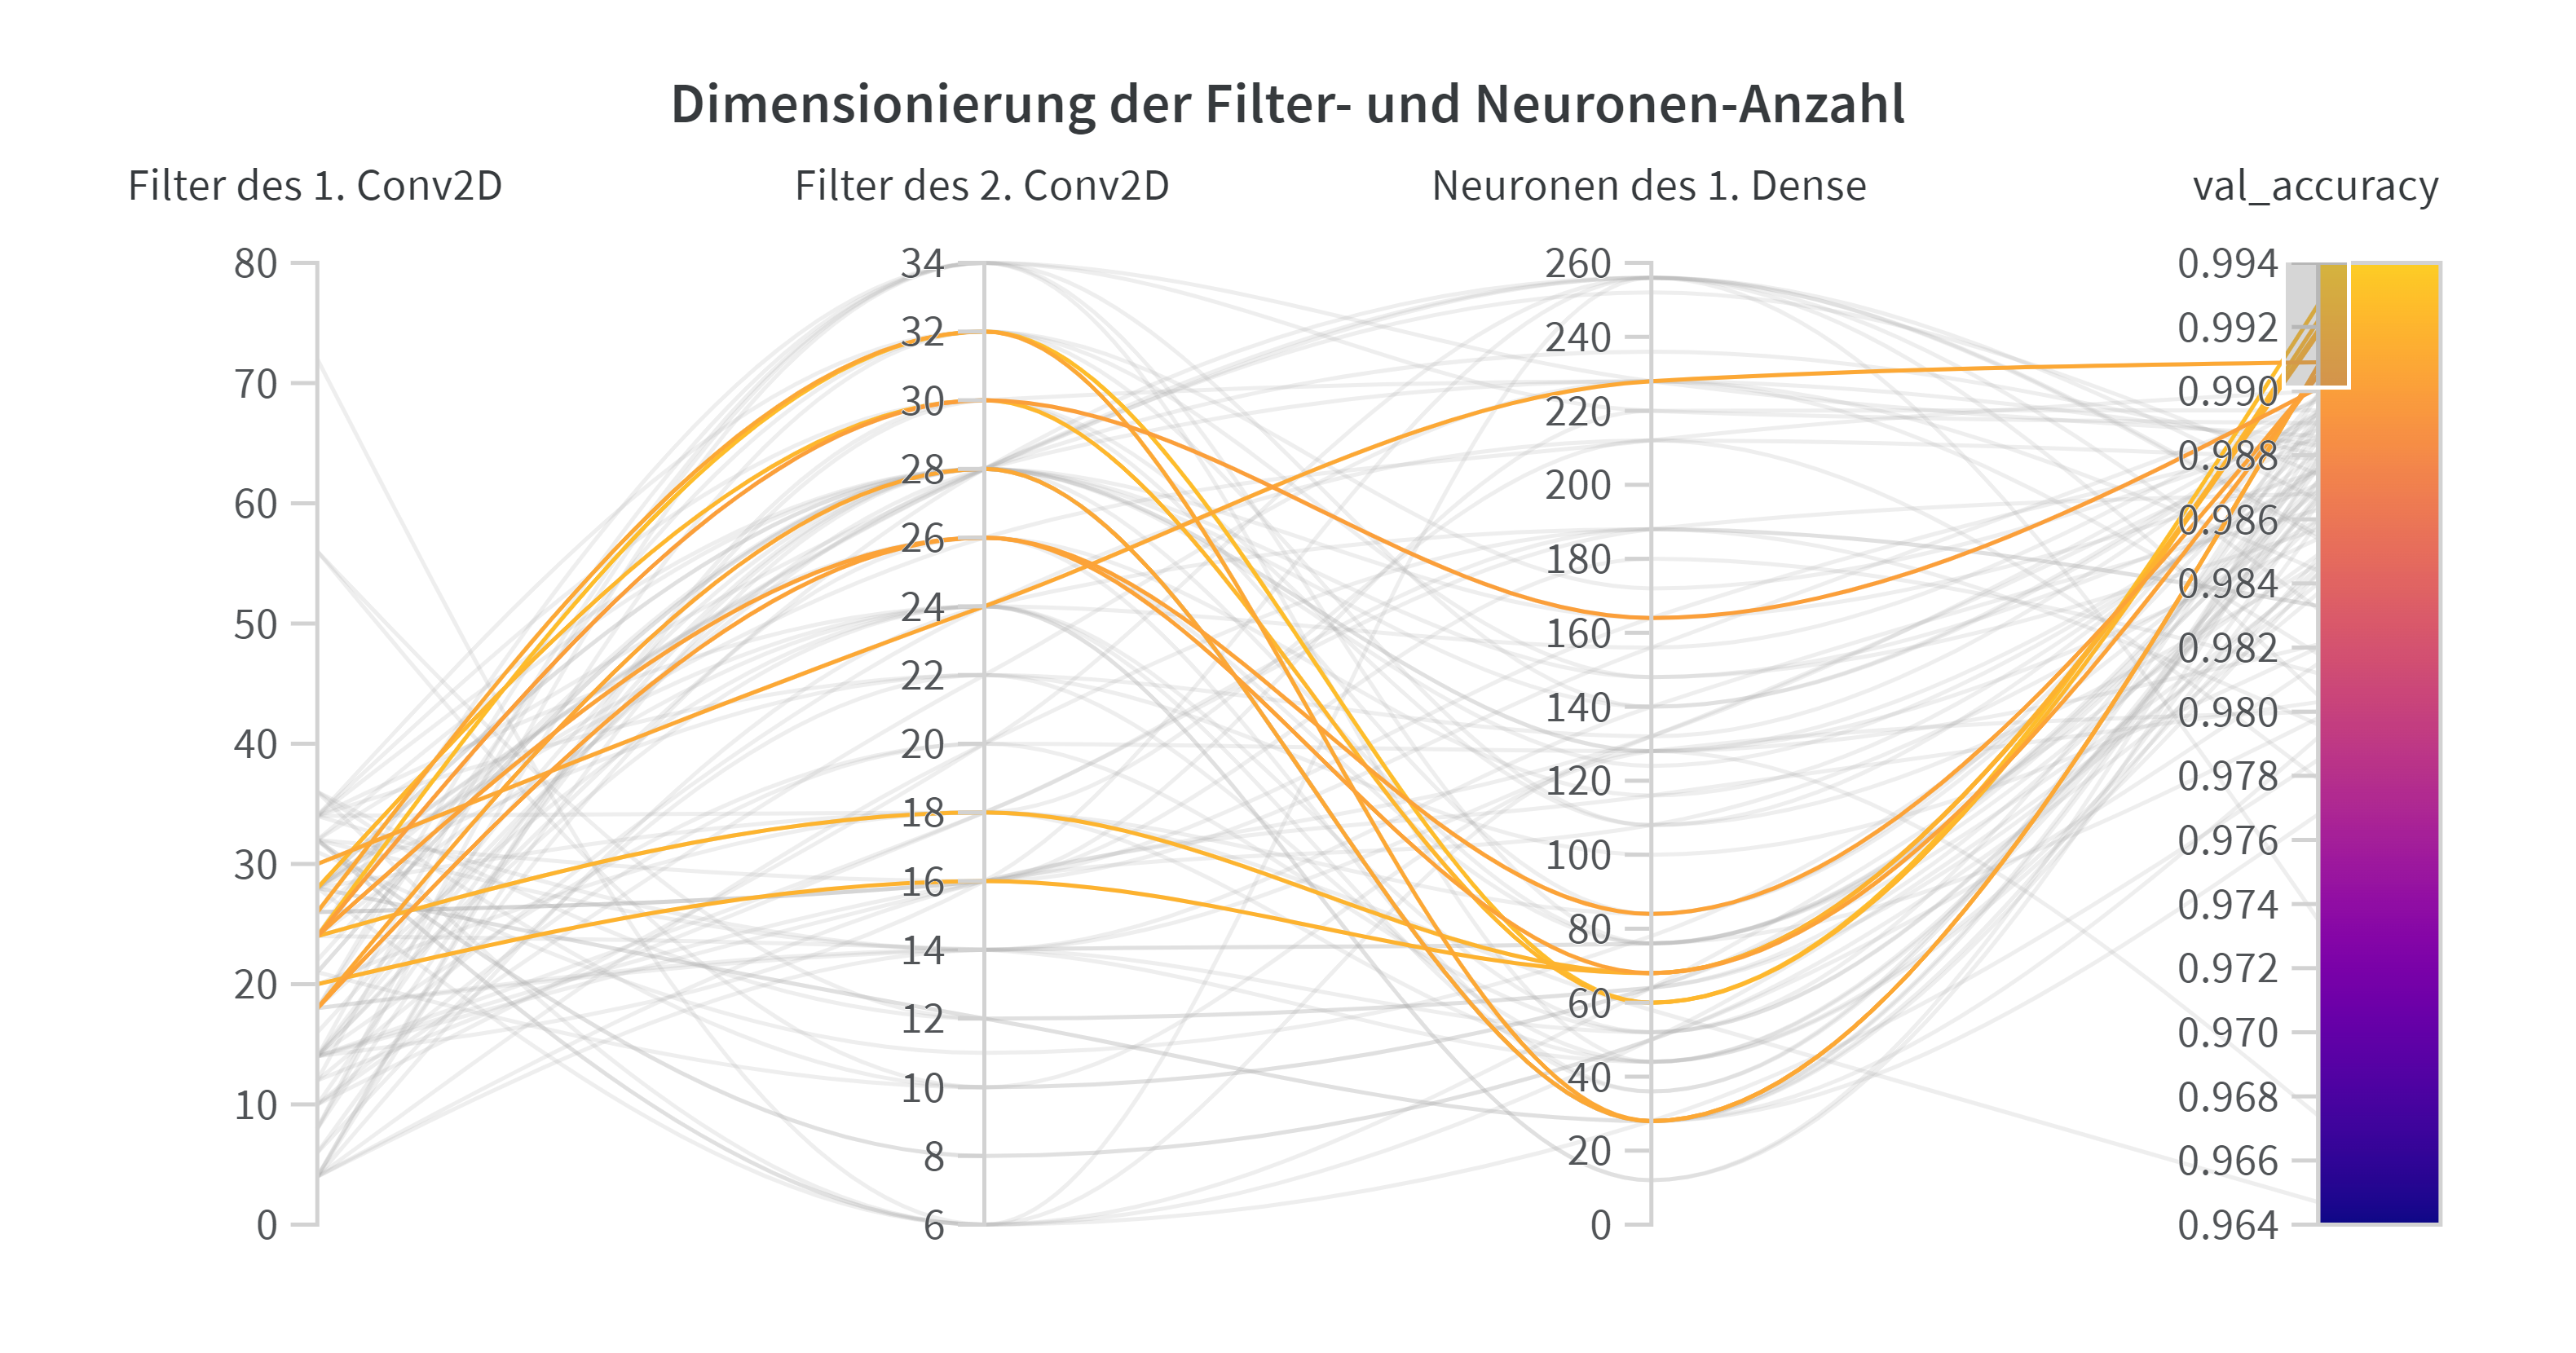
\includegraphics[width=0.7\linewidth]{images/Filter}
	\caption{2}
	\label{fig:filter}
\end{figure}

Für die Wahl wurden noch weitere Kombinationen in den eingegrenzten Bereich getestet. Schlussendlich erwiesen sich 28 Filter in beiden Convolution-Layern als erfolgreich, wodurch das Symmetrie-Bedürfnis wegen der Ähnlichkeit zur Bildgröße von 28x28 Pixeln kurzzeitig befriedigt wurde. Die Befriedigung hielt nur kurz an, da sich für die Neuronen-Anzahl 54 etablierte, was weder eine 2er-Potenz noch ein Vielfaches von 28 ist.\\

\subsection{Wahl der Aktivierungsfunktionen.}

Für die Wahl der Aktivierungsfunktionen wurden ebenfalls Sweeps durchgeführt. Die Ergebnisse sind in \autoref{fig:activ} abgebildet. Die besten fünf hervorgehoben. Sie haben die Sigmoid-Funktion im Dense-Layer gemeinsam. Bei den Convolution-Layern zeigte über alle Kombinationen hinweg die Relu-Funktion die besten Ergebnisse. Entsprechend wurde gewählt: Relu, Relu, Sigmoid.

\begin{figure}
	\centering
	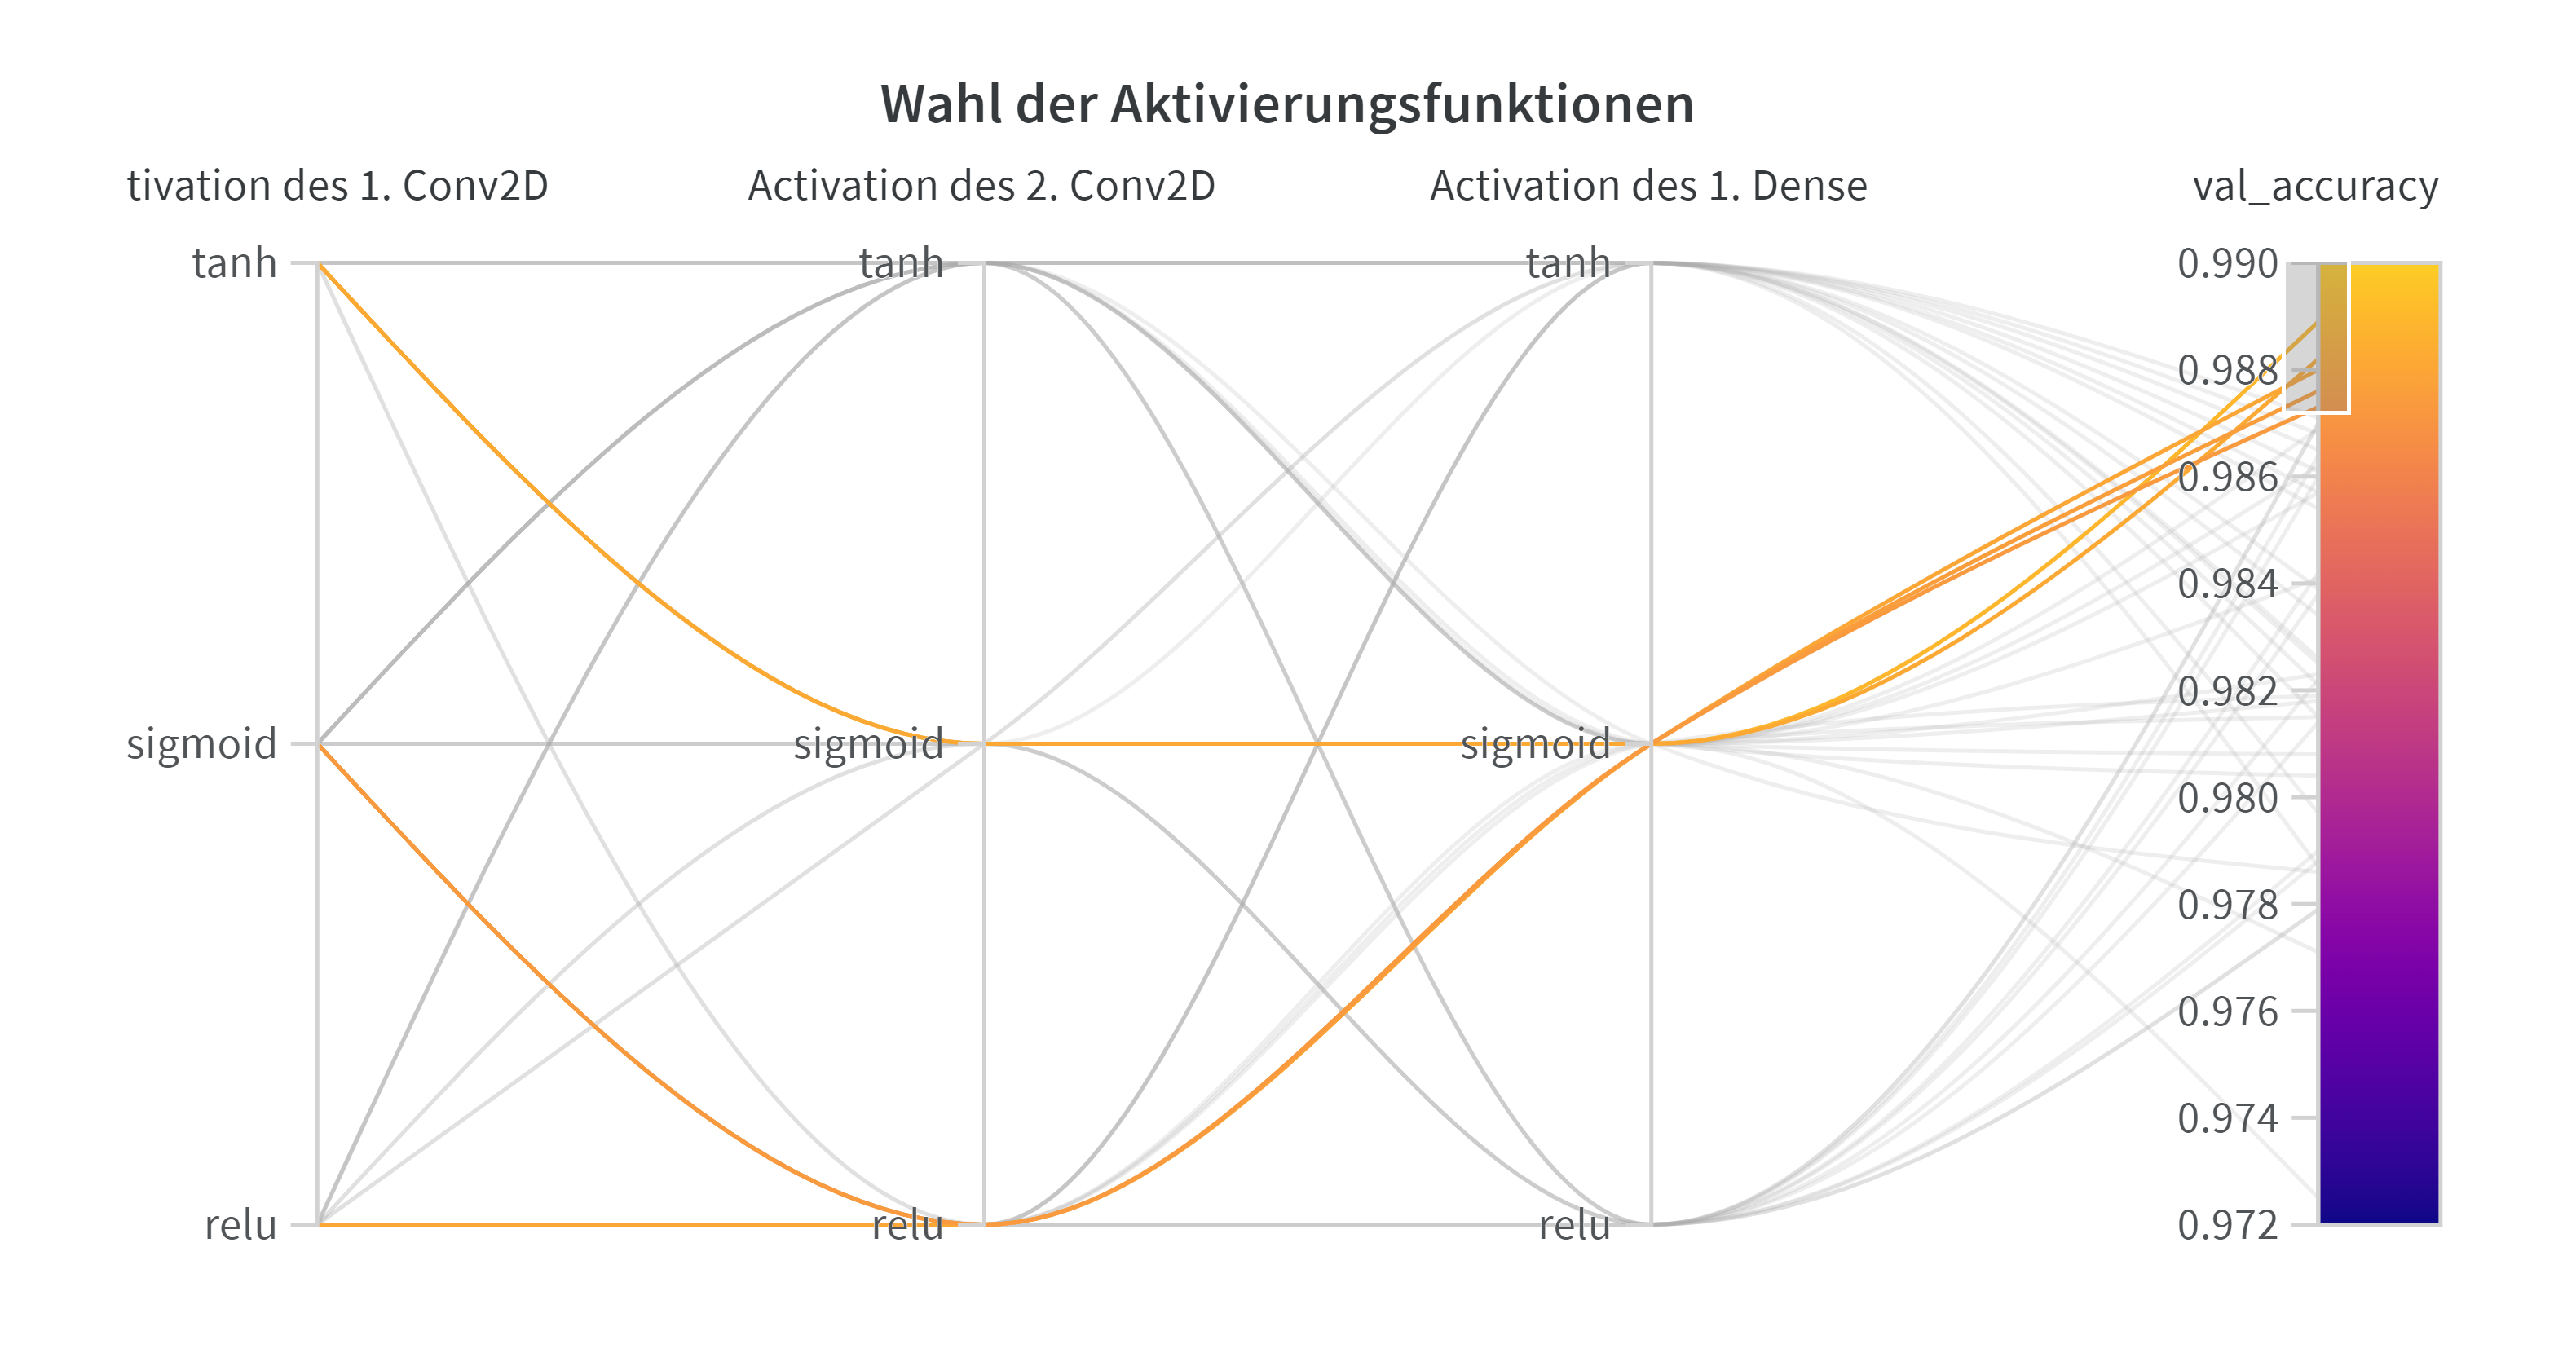
\includegraphics[width=0.7\linewidth]{images/Activ}
	\caption{1}
	\label{fig:activ}
\end{figure}

\subsection{BatchNormalization, Dropout und GaussianNoise}

\begin{lstlisting}
	tf.keras.layers.InputLayer(input_shape=(28,28,1)),
	tf.keras.layers.Conv2D(filters=28, kernel_size=5, padding='same', activation='relu'),
	tf.keras.layers.BatchNormalization(),
	
	tf.keras.layers.MaxPooling2D(2,2),
	tf.keras.layers.Dropout(0.4),
	
	tf.keras.layers.Conv2D(filters=28, kernel_size=5, padding='same', activation='relu'),
	tf.keras.layers.BatchNormalization(),
	
	tf.keras.layers.MaxPooling2D(2,2),
	tf.keras.layers.Dropout(0.4),
	
	tf.keras.layers.Flatten(),
	
	tf.keras.layers.Dense(54, kernel_regularizer = tf.keras.regularizers.l2(0.07), activation = 'sigmoid'),
	tf.keras.layers.BatchNormalization(),
	
	tf.keras.layers.Dropout(0.4),
	tf.keras.layers.GaussianNoise(0.75),
	
	tf.keras.layers.Dense(10, activation='softmax')
\end{lstlisting}


Aus insgesamt 250 Kombinationen stellte 
0.0001
256 batch
95488  params

umso enger die auswahl an hyperparemetern wurde, umso mehr epochen bis zum vergleich

Untersuchungen der Dropoutwerte zeigte Erfolg 0,4 und GaussianNoise 0.75. Hinsichtlich des papers (dropout gege noverfitting) 

sonstige versuche: adam mit sgd ersetzen erfolglos



dropout:


\section{Finale - Mit Sinn und Verständnis}

\section{Optimierung - }

Mal schauen was so kommt

\begin{lstlisting}[language=Python, caption=Python-Code, label=python_code]
	from scipy.spatial import distance
	
	x_train_best = []  # Array für die ähnlichsten Bilder
	y_train_best = []  # Array für die zugehörigen Labels
	similar_indices = [47647]  # Array für die Indizes der ähnlichsten Bilder
	
	# Berechnung der ähnlichsten Ziffern für jede Klasse von 0 bis 9
	for digit in range(10):
	
	print('Digit:', digit)
	# Filtern der Ziffern nach ihrer Klasse
	class_images = x_train[y_train == digit]
	
	# Berechnung der durchschnittlichen Cosinus-Ähnlichkeit für jede Ziffer zu anderen Ziffern derselben Klasse
	similarities = []
	for i, image in enumerate(class_images):
	avg_similarity = 0
	for other_image in class_images:
	if not np.array_equal(image, other_image):
	# Umwandlung von 28x28 Bildern in Vektoren für Cosinus-Ähnlichkeit
	image_vector = image.flatten()
	other_image_vector = other_image.flatten()
	# Berechnung der Cosinus-Ähnlichkeit
	cosine_similarity = 1 - distance.cosine(image_vector, other_image_vector)
	avg_similarity += cosine_similarity
	avg_similarity /= len(class_images) - 1  # Durchschnittliche Ähnlichkeit zu allen anderen Ziffern der Klasse außer sich selbst
	similarities.append((i, avg_similarity))
	
	# Sortieren nach der durchschnittlichen Ähnlichkeit und Auswahl der ähnlichsten Ziffer
	similarities.sort(key=lambda x: x[1], reverse=True)
	most_similar_index = similarities[0][0]
	
	most_similar_index_train_images = np.where((y_train == digit))[0][most_similar_index]
	most_similar_digit = x_train[most_similar_index_train_images]
	
	print('Index:', most_similar_index_train_images)
	
	# Hinzufügen des ähnlichsten Bildes, seines Labels und seines Index im train_images Array in den Arrays
	x_train_best.append(most_similar_digit)
	y_train_best.append(digit)
	similar_indices.append(most_similar_index_train_images)
	
	# Umwandeln der Listen in numpy arrays
	x_train_best = np.array(x_train_best)
	y_train_best = np.array(y_train_best)
	similar_indices = np.array(similar_indices)
\end{lstlisting}

24C5 means a convolution layer with 24 feature maps using a 5x5 filter and stride 1
24C5S2 means a convolution layer with 24 feature maps using a 5x5 filter and stride 2
P2 means max pooling using 2x2 filter and stride 2
256 means fully connected dense layer with 256 units


784 - [32C3-32C3-32C5S2] - [64C3-64C3-64C5S2] - 128 - 10

\section{batchsize }

während des testens 256 sinnvoll
gleicher erfolg auch mit 32 aber mehr streuung und hinsichtlich banchmark peaks gewünscht

\section{callbacks}


\section{Dropout}

Paper:
Dropout: A Simple Way to Prevent Neural Networks from
Overfitting
Nitish Srivastava nitish@cs.toronto.edu
Geoffrey Hinton hinton@cs.toronto.edu
Alex Krizhevsky kriz@cs.toronto.edu
Ilya Sutskever ilya@cs.toronto.edu
Ruslan Salakhutdinov 

\section{Variable Learning Rate}

\begin{lstlisting}[language=Python, caption=Variable Learning-Rate, label=vlr]
		vlr = tf.keras.callbacks.ReduceLROnPlateau(monitor='loss', factor = 0.95, patience=10, min_lr=0.0001)		
		vlr2 = tf.keras.callbacks.LearningRateScheduler(lambda x: 1e-3 * 0.995 ** x)
\end{lstlisting}

\section{Optimierung}

Chat GPT:
Wenn du zwei aufeinanderfolgende Convolutional Layers mit einer Filtergröße von 3x3 verwendest, wird das Netzwerk in der Lage sein, komplexere und nichtlineare Muster zu erlernen. Hier sind ein paar Gründe, warum das der Fall ist:

Receptive-Field-Erweiterung: Die Verwendung von zwei Convolutional Layers mit einer Filtergröße von 3x3 führt zu einem größeren Receptive Field im Vergleich zu einer einzelnen Schicht mit 5x5 Filtergröße. Dadurch kann das Netzwerk über einen größeren Bereich des Eingabebildes Informationen erfassen.

Mehrere Nichtlinearitäten: Jede Convolutional Layer wird durch eine nichtlineare Aktivierungsfunktion wie ReLU aktiviert. Wenn zwei 3x3 Convolutional Layers hintereinander geschaltet werden, werden zwischen den Schichten zwei Aktivierungsfunktionen angewendet, was zu einer stärkeren nichtlinearen Transformation der Eingabedaten führt.

Parameterreduktion: Zwei 3x3 Convolutional Layers haben insgesamt weniger Parameter als eine 5x5 Convolutional Layer. Weniger Parameter bedeuten weniger Berechnungen und weniger Anfälligkeit für Overfitting, da weniger spezifische Features gelernt werden müssen.

Lernen von tieferen Merkmalen: Das Stapeln von mehreren Convolutional Layers hintereinander ermöglicht es dem Netzwerk, hierarchische und abstrakte Merkmale zu lernen. Durch die schrittweise Verfeinerung der Merkmale von einer Schicht zur nächsten können komplexere Repräsentationen des Eingaberaums erzeugt werden.

Dieses Konzept der Verwendung von kleineren Filtern nacheinander anstelle eines einzelnen großen Filters wird oft in modernen Convolutional Neural Networks verwendet, um die Lernfähigkeit und Effizienz zu verbessern. Es trägt dazu bei, dass das Netzwerk tiefergehende und komplexere Muster im Eingaberaum erfassen kann.



https://doi.org/10.48550/arXiv.2202.01653 

Chat GPT:
Strided Convolution für Downsampling: Bei Verwendung einer Convolutional Layer mit Strides von 2 werden die Ausgabefeature-Maps aufgrund des größeren Schrittweitenwerts um den Faktor 2 in jeder Dimension reduziert. Das führt zu einer räumlichen Reduzierung der Feature-Maps und erzeugt somit einen Downsampling-Effekt ähnlich dem einer Max-Pooling-Schicht.

Trainierbare Downsampling-Operation: Im Gegensatz zur Max-Pooling-Schicht, die eine festgelegte Operation (Maximum aus einem Fenster) ohne trainierbare Parameter ist, ermöglicht die Verwendung einer Convolutional Layer mit Strides von 2 das Lernen von Downsampling-Operationen. Die Gewichte in der Convolutional Layer werden während des Trainings angepasst, um die beste Darstellung der Daten zu finden, während gleichzeitig eine Reduzierung der räumlichen Dimensionen erfolgt.

End-to-End-Lernen: Durch die Verwendung einer Convolutional Layer für Downsampling wird das Lernen von Merkmalen und Downsampling in einem End-to-End-Modell ermöglicht. Das Netzwerk lernt die geeigneten Filter, um Merkmale zu extrahieren, während es gleichzeitig die räumliche Dimension reduziert, ohne auf separate Schichten wie Max-Pooling zurückgreifen zu müssen.

Flexibilität und Anpassungsfähigkeit: Die Convolutional Layer mit Strides von 2 bietet Flexibilität in Bezug auf die Art des gelernten Downsampling. Das Netzwerk kann verschiedene Arten von Downsampling lernen, die möglicherweise besser zur spezifischen Datenverarbeitung passen als die festgelegte Max-Pooling-Operation.

Die Verwendung einer Strided Convolution für Downsampling bietet somit die Möglichkeit, eine lernbare Downsampling-Operation zu integrieren, die besser in das Gesamtkonzept des neuronalen Netzes eingebunden werden kann und es dem Netzwerk ermöglicht, sowohl Merkmale zu lernen als auch die Dimensionen der Feature-Maps zu reduzieren.


\section{Sonst noch}

cosinus nähste

Autoencoder

\section{Teil 2 - NLP}

Gandalf in Moria: „Im Zweifelsfall sollte man immer seiner Nase folgen …“


\end{document}
